 \documentclass{sigchi}

% Use this command to override the default ACM copyright statement (e.g. for preprints). 
% Consult the conference website for the camera-ready copyright statement.
%% \toappear{
%% Permission to make digital or hard copies of all or part of this
%% work for personal or classroom use is granted without fee provided that 
%% copies are not made or distributed for profit or commercial advantage and
%% that copies bear this notice and the full citation on the first page. To
%% copy otherwise, or republish, to post on servers or to redistribute to 
%% lists, requires prior specific permission and/or a fee.\\
%{\confname{CHI'13}}, May 5--10, 2012, Austin, Texas, USA.\\
%Copyright 2012 ACM 978-1-4503-1015-4/12/05...\$10.00.
%}

% Arabic page numbers for submission. 
% Remove this line to eliminate page numbers for the camera ready copy
%\pagenumbering{arabic}


% Load basic packages
\usepackage{balance}  % to better equalize the last page
\usepackage{graphics} % for EPS, load graphicx instead
\usepackage{times}    % comment if you want LaTeX's default font
\usepackage{url}      % llt: nicely formatted URLs
\usepackage{multirow} % multirow tables

% llt: Define a global style for URLs, rather that the default one
\makeatletter
\def\url@leostyle{%
  \@ifundefined{selectfont}{\def\UrlFont{\sf}}{\def\UrlFont{\small\bf\ttfamily}}}
\makeatother
\urlstyle{leo}


% To make various LaTeX processors do the right thing with page size.
\def\pprw{8.5in}
\def\pprh{11in}
\special{papersize=\pprw,\pprh}
\setlength{\paperwidth}{\pprw}
\setlength{\paperheight}{\pprh}
\setlength{\pdfpagewidth}{\pprw}
\setlength{\pdfpageheight}{\pprh}

% Make sure hyperref comes last of your loaded packages, 
% to give it a fighting chance of not being over-written, 
% since its job is to redefine many LaTeX commands.
\usepackage[pdftex]{hyperref}
\hypersetup{
pdftitle={SIGCHI Conference Proceedings Format},
pdfauthor={LaTeX},
pdfkeywords={SIGCHI, proceedings, archival format},
bookmarksnumbered,
pdfstartview={FitH},
colorlinks,
citecolor=black,
filecolor=black,
linkcolor=black,
urlcolor=black,
breaklinks=true,
}

% create a shortcut to typeset table headings
\newcommand\tabhead[1]{\small\textbf{#1}}


% End of preamble. Here it comes the document.
\begin{document}

\title{Carp\'{e} Data: Supporting Serendipitous Data Integration in Personal Information Management}

\numberofauthors{3}
\author{
  \alignauthor 1st Author Name\\
    \affaddr{Affiliation}\\
    \affaddr{Address}\\
    \email{e-mail address}\\
    \affaddr{Optional phone number}
  \alignauthor 2nd Author Name\\
    \affaddr{Affiliation}\\
    \affaddr{Address}\\
    \email{e-mail address}\\
    \affaddr{Optional phone number}    
  \alignauthor 3rd Author Name\\
    \affaddr{Affiliation}\\
    \affaddr{Address}\\
    \email{e-mail address}\\
    \affaddr{Optional phone number}
}

% Teaser figure can go here
%\teaser{
%  \centering
%  
\includegraphics{Figure1}
%  \caption{Teaser Image}
%  \label{fig:teaser}
%}

\maketitle

\begin{abstract}
Exploratory sequential mixed-method study
\end{abstract}

\keywords{}

\category{H.5.m.}{Information Interfaces and Presentation (e.g. HCI)}{Miscellaneous}

\terms{Human Factors; Design; Measurement.}

\section{Introduction}

In recent years, an unprecedented quantity and variety of information has been made available as structured data on the Web, through APIs, datasets, and data feeds.  This information includes: access to data previously hidden behind services and applications, such as retailer product catalogues; information not previously directly released to the public, such as open government data or records of personal financial transactions; and new kinds of data generated by emerging kinds of data sources, such as wearable and smartphone-based biosensors.  A primary goal of opening up this data is that end-user citizens can make more informed decisions pertaining to their health, wealth, and well-being \cite{}.  This data is predominately used by specialised app developers, journalists and other ``data specialists'' but remains inaccessible to citizens because of the available tools.  For example, the most commonly used structured personal information management (PIM) tools either manage a small, fixed set of data types (such as digital calendaring tools and  to-do list managers) or provide little or no support for structured data at all, such as text editors and sketching/drawing tools \cite{}.   

We hypothesise that end-users will benefit from tools that allow them effectively browse, use and consume heterogeneous structured data from diverse sources. In this paper, we present an investigation into extending PIM tools to effectively use emerging ecosystems of personal data.  We used a three-stage sequential exploratory mixed-method approach: first, we performed a qualitative analysis of a semi-structured interview pre-study to understand the types of tasks people performed using a plurality of information sources, and the processes that they relied upon to perform such tasks.  Our results suggested that people rely on multiple and diverse sources, then singular, integrated ones for a number of reasons, including coverage, reliability, and for alternative perspectives.  

% Second, we conducted a quantitative, structural analysis of various popular personal data sources available today to identify potential barriers to effective unification of data.  Drawing upon definitions from the database integration and automatic schema matching literature, we characterised the types of heterogeneity exhibited across data sources in six domains: address books (contact info), event calendars (events), music (songs/tracks), shopping (product info) social networking (profiles) and weather (forecasts), finding that terminological heterogeneity dominates the simpler data feeds (including social networking and restaurant recommendations), while structural issues pervade the more complex schemas of online retailers' product catalogues.

Second, we conducted a structural analysis of various popular personal data sources available today to identify potential barriers to unifying data.  Drawing upon definitions from the database integration and automatic schema matching literature, we characterised the types of heterogeneity exhibited across data sources in six domains: contacts, events, music, shopping, social networking and weather, finding that terminological heterogeneity dominates the simpler data feeds (including social networking and restaurant recommendations), while structural issues pervade the more complex schemas of online retailers' product catalogues.


Third, we developed DataPalette, an interface that enables serendipitous ``data mixing,'' negating the need for people to write bespoke code to effectively combine and compare heterogenous data.  It was principally designed to support people's data integration needs for data heterogeneity, using observations made from the previous studies.  In particular, we designed a user-centric interface to facilitate simple, ``light-touch'' integration tasks of diverse, heterogeneous data sources.  We then performed a usability evaluation of DataPalette, which revealed that most users were comfortable with the interactive integration mechanisms we devised, and that this interface effectively improved people's ability to perform multifaceted decision making tasks using multiple sources.

\section{Background}

In this section, we motivate our work using three fields: PIM, data integration, and end-user mashups and toolkits.  Our primary motivation stems from field studies in PIM, where consolidating and working with data from multiple sources has remained a challenge for over a decade. Enabling PIM tools to supporting ad-hoc data integration has remained difficult because of the complex, theoretically difficult nature of data heterogeneity; specifically, reconciling the differences that arise among representations when data is created by different people, at different times, for different purposes. As described by Alon Halvey:

\begin{quote} 
  The problem stems from the fact that] we are trying to integrate data systems that were developed for slightly (or vastly) different business needs. Hence, even if they model overlapping domains, they will model them in different ways. Differing structures are a byproduct of human nature --- people think differently from one another even when faced with the same modelling goal~\cite{alonhalevy}.\looseness=-1
\end{quote}

Recently, users are experiencing data fragmentation~\cite{Jones05towardsa} across multiple web-based applications and services, and struggle to consolidate across them~\cite{bergman,boardmansasse}.  In our own previously-conducted field study, (reference anonymised) we observed variations of manual ``coping strategies'' (or, if programmers, elaborate, custom-coded one-off solutions) to allow people to manage both online and offline data.  Similar findings from other studies include Voida et al.'s observations of volunteer coordinators' ``homebrew databases'', manually-maintained information assemblages concocted to handle the widely varied and heterogeneous data collection requirements such groups needed to coordinate their activities \cite{Voida:2011:HDC:1978942.1979078}.










%In this section, we motivate our work using three fields: PIM, data integration, and end-user mashups and toolkits.  Our primary motivation stems from field studies in PIM, where consolidating and working with data from multiple sources has remained a challenge for over a decade. Recently however, users are experiencing data fragmentation~\cite{Jones05towardsa} across multiple web-based applications and services, and struggle to consolidate across them~\cite{bergman,boardmansasse}.  In our own previously-conducted field study, (reference anonymised) we observed variations of manual ``coping strategies'' (or, if programmers, elaborate, custom-coded one-off solutions) to allow people to manage both online and offline data.  Similar findings from other studies include Voida et al.'s observations of volunteer coordinators' ``homebrew databases'', manually-maintained information assemblages concocted to handle the widely varied and heterogeneous data collection requirements such groups needed to coordinate their activities \cite{Voida:2011:HDC:1978942.1979078}.
%% TODO MORE HERE

%% don't like the beginning of this > 
%Enabling PIM tools to supporting ad-hoc data integration has remained difficult because of the complex, theoretically difficult nature of data heterogeneity; specifically, reconciling the differences that arise among representations when data is created by different people, at different times, for different purposes. As described by Alon Halvey:

%\begin{quote} 
  %The problem stems from the fact that] we are trying to integrate data systems that were developed for slightly (or vastly) different business needs. Hence, even if they model overlapping domains, they will model them in different ways. Differing structures are a byproduct of human nature --- people think differently from one another even when faced with the same modelling goal. \cite{alonhalevy}
%\end{quote}

% i think we do not need to differentiate between semantic web and databse integration here, we're saying they're both bad, let's lump them together to keep the argument flowing and not kill our readers
The database integration and Semantic Web \cite{Shadbolt:2006:SWR:1155313.1155373} research communities have primarily focused efforts on purely-automatic approaches to the problem of data integration.  Such approaches typically take the form of either \emph{ontology} or \emph{schema-level matching}, or \emph{direct} or \emph{instance-level} matching.  We presently focus  on \emph{instance-level} matching, as schemas may not always be available, nor easily accesssed by users. Approaches to automatic instance matching have included applied natural language processing (NLP) techniques for terminological matching (e.g., \cite{euzenat2004api}), machine-learning techniques that use both structural and terminological features for matching \cite{doan2003learning}, probabilistic approaches \cite{suchanek2011paris}, and instance schema comparisons using structural and logical definitions \cite{castano2006matching}.   In real-world settings, however, manual and semi-automatic matching approaches are favoured over automatic because of the need for high degrees of accuracy.  

A different approach entirely has been taken in the web mash-up community; this community has largely focused on end-user interfaces that allow people to interactively reconcile data from multiple sources.  Yahoo Pipes! is a visual programming language aimed at letting novice programmers easily create data-transformation workflows, but remained rather challenging to  use and effort-intensive for one-off information tasks.  Mash-up makers such as Intel Mashmaker \cite{}, QDEWiki \cite{}, and TX2 \cite{}. DataPalette's approach is most directly inspired by ``lightweight'' visual, user-interactive data collection, consolidation and alignment tools such as Potluck \cite{citeulike:3875264} and Cards \cite{Dontcheva:2007:RCS:1294211.1294224}.

% Semi-automatic approaches use varying levels of support to aid a user, from prompting users to manually check flagged alignments, to suggesting possible alignments.  Allowing users to compare instances across heterogeneous data is powerful because users can combine and evaluate multiple sources.  In principle, automatic instance matching approaches would allow users to seamlessly browse this data, however for now and the foreseeable future such approaches cannot make use of personal knowledge and do not guarantee their alignments.  Therefore, in our work, we adopt a semi-automated matching approach, which will support the user to make alignments between web data and their personal data.

A number of research PIM systems have demonstrated a great number of ways that users could benefit from better support for data integration.  For example, SEMEX's \cite{semex} rich uniform query interface allowed users to quickly trace references of people, places and things across files, folders and repositories.  Similarly, Haystack, a personal information platform, allowed users to visualise and customise how they worked with their data in a uniform, consolidated manner \cite{haystack}. Pertaining to each system's ability to integrate information from arbitrary new data sources, however, both systems generally required new sources to either already conform to a pre-specified set of ontologies, or have the user provide a manual specify such a mapping translation themselves.


% integrated into the above :: 

%% The Semantic Web research community has approached the problem of data integration in terms of \emph{ontology matching}, which can be split into two distinct strategies: \emph{schema} and \emph{instance} matching.  Instance matching differs from schema level matching in that it aims to detect instances referring to the same real world object, while schema matching aims to find a set of mappings between concepts and properties in different ontologies. For our purposes of allowing users to explore and compare data from different websites, we are particularly interested in aligning instances of the most common forms of data that people compare from website to website.  
%% Instance matching within this scope is in its infancy, some of its problems have been addressed by the record linkage problem in the database field \cite{fellegi1969theory,winkler1999state,gu2003record}.  However, there are new problems to address in this field, which are strongly related to schema matching, including structural heterogeneity and logical heterogeneity. The approaches used to match instances typically use: natural language processing, using lexicons like Wordnet\footnote{\emph{Wordnet} - \url{http://wordnet.princeton.edu}} to identify synonyms, and word stems \cite{euzenat2004api}; machine learning techniques \cite{doan2003learning}; probabilistic approaches \cite{suchanek2011paris} and comparisons of instance schemas structural and logical definitions \cite{castano2006matching}.  In our case, this is problematic because information from the web does not always have a schema.  In real-world scenarios, semi-automatic ontology matching approaches are favoured over automatic because reconciling the differences between ontologies that were designed for different purposes is not always accurate.  Semi-automatic approaches use varying levels of support to aid a user, from prompting users to manually check flagged alignments, to suggesting possible alignments.  Allowing users to compare instances across heterogeneous data is powerful because users can combine and evaluate multiple sources.  In principle, automatic instance matching approaches would allow users to seamlessly browse this data, however for now and the foreseeable future such approaches cannot make use of personal knowledge and do not guarantee their alignments.  Therefore, in our work, we adopt a semi-automated matching approach, which will support the user to make alignments between web data and their personal data.
%% The Semantic Web community use ontologies to formally describe vocabularies for specific domains by defining axioms describing entities, instances of entities and the relationships that hold among them \cite{borst1997construction}. The axioms in an ontology can be either assertional or terminological, the former describes the schema of the entities and the latter the instances of those entities. Typically, these ontologies are marked up using OWL (Web Ontology Language) and Resource Description Framework Schema (RDF(S)).  There has been an explosion of ontologies published online, many of which describe the same entities.  These entities may or may not share the same entity names or properties.  Therefore using data from heterogeneous ontologies can be difficult. The field of ontology matching can be split into two fields: schema and instance matching.  Instance matching differs from schema level matching, because it aims to detect instances referring to the same real world object, while schema matching aims to find a set of mappings between concepts and properties in different ontologies.
% For our purposes of allowing users to explore and compare data from different websites, we are particularly interested in aligning instances of the most common forms of data that people compare from website to website.  Instance matching within this scope is in its infancy, some of its problems have been addressed by the record linkage problem in the database field \cite{fellegi1969theory,winkler1999state,gu2003record}.  However, there are new problems to address in this field, which are strongly related to schema matching, including structural heterogeneity and logical heterogeneity.
% The approaches used to match instances typically use: natural language processing, using lexicons like Wordnet to identify synonyms, and word stems \cite{euzenat2004api}; machine learning techniques \cite{doan2003learning}; probabilistic approaches \cite{suchanek2011paris} and comparisons of instance schemas structural and logical definitions \cite{castano2006matching}.  In our case, this is problematic because information from the web does not always have a schema.  In real-world scenarios, semi-automatic ontology matching approaches are favoured over automatic because reconciling the differences between ontologies that were designed for different purposes is not always accurate.  Semi-automatic approaches use varying levels of support to aid a user, from prompting users to manually check flagged alignments, to suggesting possible alignments.  Allowing users to compare instances across heterogeneous data is powerful because users can combine and evaluate multiple sources.  In principle, automatic instance matching approaches would allow users to seamlessly browse this data, however for now and the foreseeable future such approaches cannot make use of personal knowledge and do not guarantee their alignments.  Therefore, in our work, we adopt a semi-automated matching approach, which will support the user to make alignments between web data and their personal data.

\section{Pre-studies: The Need for and Challenges in realizing Ad-Hoc Data Integration in PIM Tools}

%% not sure where this goes >> but i want to keep it

We performed an exploratory sequential mixed-method study to help us design our contribution. For our first pre-study, we first sought an updated understanding of how and whether people still used multiple information sources regularly when they sought information on the Web. There were two reasons for this inquiry; first, whether people were increasingly either relying only on the handful of the massive ``supersites'' (Facebook, Google, Wikipedia) for most of their activities, or searching across distributed sources of information.  If this were the case, much of the benefit could be gained by merely integrating PIM tools with the handful of sites, rather than the substantially more challenging problem of integrating data from arbitrary information sources on the Web.   Second, whether people relied on multiple sites and why.  If they did what kinds of tasks did people required diverse information collection and were these kinds of tasks rare?  If so, this would suggest that perhaps specialised interfaces could be concocted for this purpose rather than it being a PIM need. 

The second pre-study focused on the characteristics of the data available from the kinds of sites used by the first pre-study's participants for the tasks described. The purpose of this follow-on  was to identify not specific characteristics of particular sites in question, but to identify, in general, the degree of complexity of the data feeds currently available across a variety of domains, and typical integration problems that might arise when mixing this data. The next two sections, we present our methodologies and results for our pre-studies.


\subsection{PS.1 - Understanding Data Diversity in Everyday Tasks}
We designed a semi-structured interview about tasks people performed online that required the use of multiple websites, and the processes people used to perform such tasks.  We analysed the data collected from this study using a thematic approach.  In our pre-study, we investigated the types of tasks people performed online that required heterogeneous data sources, and which tools they would use to organise a social event involving around 15 people.  We planned to interview 8 participants, using a general interview guide approach based on a set of questions.  This approach allowed the interviewer to adapt the interview to the participant's experiences, while collecting the same general areas of information.  Each interview was recorded and notes taken, the interviewer was trained in the purpose of the study and to minimise bias.


\subsubsection{Results}
The participant demographic consisted of 8 people (7 male and 1 female).  They were split evenly into two age groups of 18-25 and 26-32.  All but one participant reported they used social network sites very regularly (many times a day); they said they either logged in multiple times a day, left a website page open or used dedicated application for their social networking site updates.  Those that used social networking websites primarily used Facebook.  All of the participants used Twitter to listen to broadcasted tweets, and 6 out of 8 people regularly tweeted.  The following two sections, describe the tasks people perform online with heterogeneous data and how they would use to organise a large social event.

\subsubsection{Question 1: Heterogenous Data Tasks}
All participants reported having used multiple websites to accomplish a task.  They listed example tasks such as shopping (including food, consumer electronics, hotels and flights), choosing restaurants, searching for jobs, when choosing a university, choosing recipes, study and work.  The biggest focus for shopping focused tasks was balancing price, quality and speed of delivery.  In general, people did not not trust a single websites for reviews because they said that they could be biased and did not always review the features they were interested in.  One participant said that video reviews of items were really important because they showed the aesthetics and scale of the item.  In general for initial research into organising a task it was typical to Google keywords to find related websites to their tasks.  They identified that they used different website for different jobs, such as manufacturers website for technical details, review aggregators for a range of opinions, and Google maps for location based decisions.  Social networks were also identified to have different functions, such as different groups of people belong to each and share different types of opinions.  One participant said that they shared their outlook and gmail calendars, but only for work events and did not record social activities on them.

\subsubsection{Question 2: Process Used to Organise a Large Social Event}
All of the participants would organise a large social event by talking to their friends, about their ideas, preferences and recommendations.  The tools they would use to acquire this information included face-to-face, phone calls, email, Skype, Facebook events.  The method chosen depended on the time scale required to organise an event, in general if there was a short time scale people would speak in person or on the phone.  Otherwise, people would set up a Facebook event page to discuss ideas with their friends.  If their friends were not on Facebook they would email them.  All but one participant said they would not use Doodle\footnote{Doodle - \emph{www.doodle.com}} to the organise day and time of an event, because they felt that people did not fill in the form and it was more suit to organising work events.  

Most people felt that being assertive and posting their decisions about the date and time on Facebook meant that organising events were more successful than trying to gather a consensus.  They expected that their friends would voice any objections if they could not attend or like the restaurant or activity selected.   They selected venues, locations, restaurants and activities based on their own knowledge, friend's recommendations, Google maps, reviews obtained through web search and sites such as TripAdvisor.  People stated that the cost, price and easy to get to locations were the most important factors when choosing a venue.  They considered how to get there and looked up train or bus times on the Web, or organised carpools.  When organising an event the weather was not that important because they did not trust the accuracy of predictions.  Also, their friend's preferences in price and food choices were not a priority; they would try to be inclusive but only if it meant small changes to the plan.  Choosing food and timings were often made on-the-fly, by either with the use of mobile applications or by walking past a location.

\subsubsection{Summary of Findings}
People said that they would like a website that could support the evolution of an event, that allowed them to post drafts of an event.  They felt that organising an event should be a process that changes over time.  Three participants said that they would like a recommendation system for places to eat and activities.  Another strong requirement was that it had to be ubiquitous so that everyone could use it because they wanted a single place to communicate with their friends.  While Facebook was the most popular social networking site for organising events, half of the participants felt that it was not the best solution and would prefer a collaborative environment.

\begin{table*}
\small
\begin{tabular}{p{2.0cm}  p{1.8cm}  p{1.8cm}  p{1.8cm}  p{1.8cm}  p{1.8cm}  p{1.8cm}  p{1.8cm}}
				&				& {\bf average}				& {\bf average }				& 				& {\bf prop name}			& {\bf structural} 			& {\bf model } \\
				& {\bf source}		& {\bf props/record}			& {\bf depth/record}			& {\bf equivalent to}	& {\bf inconsistent}			& {\bf inconsistency} 			& {\bf inconsistency} \\
\hline
social networking	& google+			& 12						& 1.52					& tw:5, li:4, fb:4		& tw:3, li:2, fb:2				& tw:0, li:1, fb:1				& tw:0, li:0, fb:0 \\
(profiles)			& twitter			& 39						& 1.37					& li:4, fb:4 			& li:2, fb:1					& li:0, fb:0					& li:0, fb:0 \\
				& linkedin			& 18						& 2.42					& fb:7			& fb:5					& fb:3					& fb:0 \\
				& facebook		& 22						& 1.5						&				&						&						& \\
\hline
calendars			& google calendar	& 15						& 1.46					& eb:9			& eb:6					& eb:1					& eb:1 \\
(events)			& eventbrite		& 32						& 1.43					&				&						& 						& \\
\hline
retail				& milo			& 5						& 1.2						& z:2, s:3, e:1, a:3	& z:2, s:2, e:1, a:3			& z:0, s:0, e:0, a:2			& z:0, s:0, e:0, a:0 \\
(products)			& zappos			& 6						& 1						& s:2, e:2, a:3		& s:2, e:2, a:2				& s:0, e:0, a:0				& s:0, e:0, a:0 \\
				& shopping.com	& 11						& 3.74					& e:2, a:8			& e:2, a:8					& e:0, a:0					& e:0, a:0 \\
				& etsy			& 31						& 1.13					& a:11			& a:10					& a:1						& a:2 \\
				& amazon			& 108					&						&				& 						&						& \\
\hline
contacts			& google contacts	& 7						& 1.46					& yp:2			& yp:2					& yp: 0					& yp: 0 \\
				& yellowpages		& 25						& 1						&				&						&						& \\
\hline
music			& echonest		& 4						& 1.83					& so:3, r:3, sp:3		& so:3, r:3, sp:3				& so:0, r:0, sp:0				& so:0, r:0, sp:0 \\
(songs/			& soundcloud		& 42						& 2.14					& r:12, sp:7		& r:11, sp:6 				& r:1, sp:1					& r:1, sp:0 \\
tracks)			& rdio			& 27						& 2						& sp: 7			& sp: 6					& sp: 1					& sp: 1 \\
				& spotify			& 10						& 2.44					&				&						&						& \\
\hline
weather			& weatherbug		& 8						& 2						& wu: 5, y: 5		& wu: 5, y: 5				& wu: 5, y: 4				& wu: 0, y: 0 \\
(forecasts)		& wundergound	& 52						& 1.38					& y:12			& y:12					& y:7						& y:3 \\
				& yahoo weather	& 22						& 1.58					&				&						&						& \\
\end{tabular}
\caption{\emph{PS.2 Results} - Analysis of heterogeneity present across data feeds, by category of feed}\label{tbl:prestudy2}
\end{table*}


\subsection{PS.2 - Technical Challenges of Data Integration}
Our investigation of integration challenges of available structured data feeds started with identifying a set of candidate sources to examine.  For this, we consulted the ProgrammableWeb API directory\footnote{ProgrammableWeb - \url{http://www.programmableweb.com/apis/directory}} of 50 most popular data feeds measured by the number of developer API keys issued for each.  To increase the variety of sources, we first categorised sources into 5 topic categories: social network services, retailers, event sources (e.g., online calendars and event sites) music, and weather, and selected 2-5 sources from each 2-5 feeds each for a total of 20 total feeds for analysis.  

For each feed, 3-5 ``typical'' records of a single type were obtained; for social networking sites this was user profiles, for music sites this was song info, etc.  Records were located either by first querying for popular key terms using each site's keyword query API (if available), or a ``top products'' query if available.  For each obtained data record, two simple complexity metrics were computed: an \emph{average width} and \emph{average depth} of record.  For determining the width, we first examined the record to find the appropriate level for comparison; for example, Amazon's retail product ``Item'' root record had few attributes about the actual product compared to its ``ItemAttributes'' sub-property, which was used instead. Thus, all comparisons were made to maximize comparative similarity.  Depth was computed as the average number of levels from record root to leaves across all properties, and was measured, with width, to convey the overall size/complexity of each record.

The third metric measured the amount of overlap among the sources in each category.  This was done by determining \emph{equivalent properties} between schemas, which we did manually by creating an alignment table for all properties across all data sources in each category.  Each row of the alignment table comprised a property of a record from one data source, and all its closest matching properties from the others.  We used both property names and attribute descriptions (in documentation, if available) to make matching decisions; two properties were aligned if they seemed to model the same piece of information.

Once the equivalent properties were established, we look at how many of these properties were terminologically inconsistent, that is, identified using different property names.   Then, ignoring property name, we looked to see if its values were structurally comparable.  If two fields were of the same data type and, if complex, had equivalent subfields, they were considered comparable; otherwise they were considered \emph{structurally inconsistent}.  An example of such a structural inconsistency were``birthday'' fields in Facebook and LinkedIn; Facebook represented it as a single string formatted ``MM/DD/YYYY'', while LinkedIn represented it as a sub-structure with separate ``Month'', ``Day'' and ``Year'' subfields.  

Finally, we looked at fields that were equivalent, yet which could not be compared for reasons other than the terminological and structural reasons above.  These \emph{modelling differences} were caused by a variety of reasons including, but not limited to, the following: measurement unit inconsistencies, how data was measured (e.g., dewpoint vs relative humidity), differences in scale or granularity, and mismatches in what was being modelled (``offer'' versus ``listing'').

\subsubsection{Results}
Table \ref{tbl:prestudy2} displays the raw results of the process just described.  A number of features were quite striking about the data. First, while most of the data records were small and relatively simple, nearly one in each category produced substantially more complex records than the rest; in particular, Amazon, Soundcloud, Twitter and Weather Underground stood out in their respective categories. 

Looking at overlap, we notice overall little overlap among records; that is, except for the smallest records (which had few properties to begin with), most of the data records had more unique properties than ones in common with others.  While some of these 'unique records' were primarily for internal, service-specific use (such as service-specific IDs) others were useful properties one would expect to find in a record that were simply not present.  Only one of the music data providers, Spotify, included information about the album(s) that featured a particular song.  Such omissions show us that these data APIs reflect each service provider's own capabilities and internal data representations very specifically, and that integrating data such records from multiple sources could allow more complete and useful representations to be assembled.

The second finding is that equivalent properties were sometimes, though only rarely, given the same name.  Thus, terminological heterogeneity was prevalent across data records we observed.  Structural heterogeneity, however, was comparatively rare, with the most common case being similar to the birthday example above; a leaf property on one record modeled as a subtree in the other.  We also encountered, particularly in the Weather category, examples of fields which had data embedded in textual description fields 

%\section{Designing the DataPalette Interface}
\section{Designing DataPalette : An Interface for Serendipitous Data Mixing}
\begin{figure*}[tbp]
\begin{center}
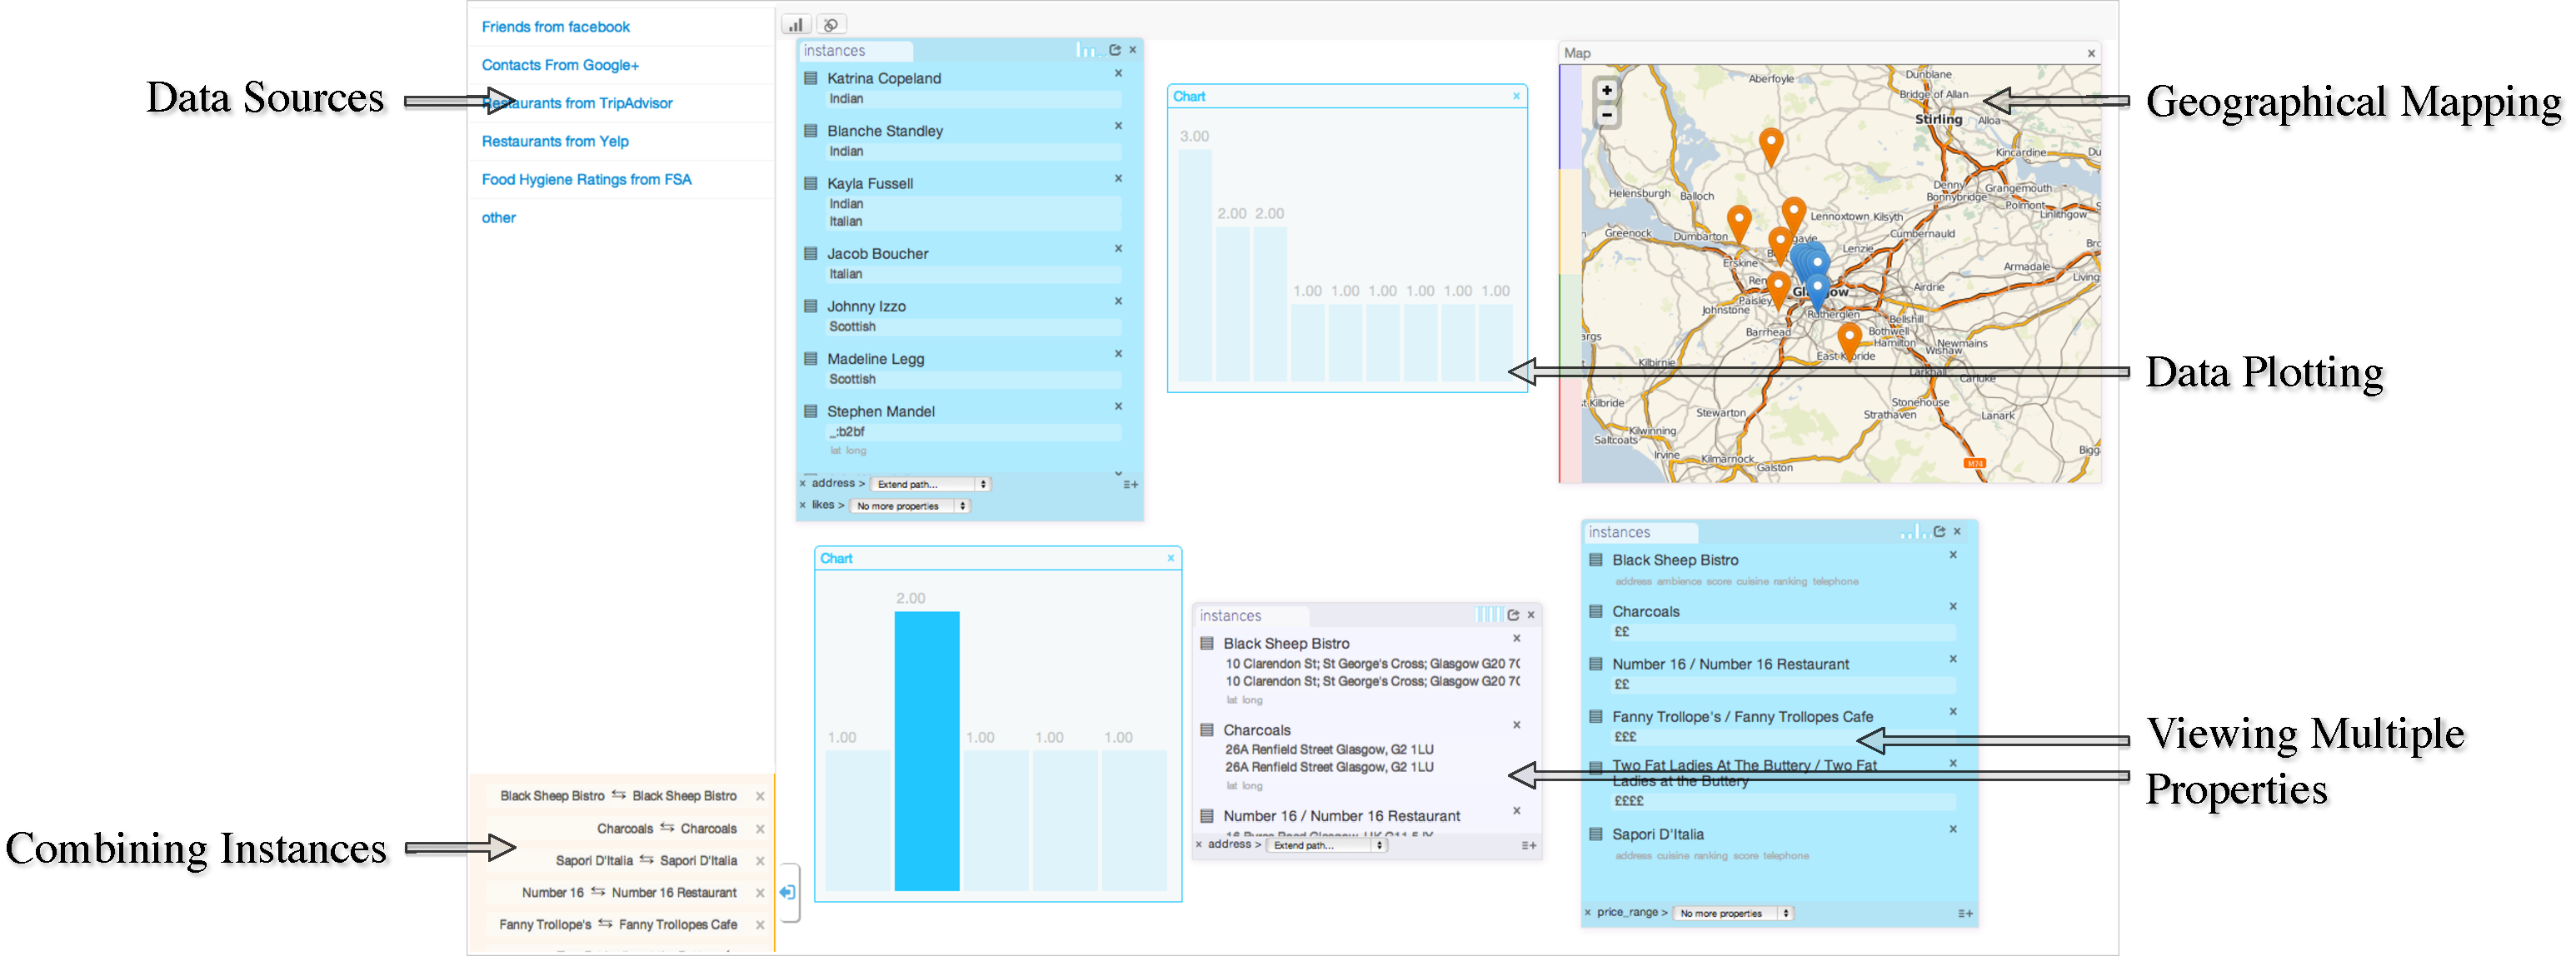
\includegraphics[width=18cm]{img/screenshot}

\caption{DataPalette Workspace, a file manager-inspired Drag and Drop interface for structured data mixing. Collapsible displays of data sources are listed on the left, from which instances or entire sets of items can be dragged to form a window (group) on the workspace.}

\label{fig:workspace}
\end{center}
\end{figure*}

At a high level, the overall goal of DataPalette was to empower end-users to mix arbitrary structured data feeds on-the-fly while solving their particular information task(s) - be them sense-making or decision-making related - in order to more effectively accomplish these tasks.  Unlike Mashup makers, including Yahoo Pipes!, the goal was to facilitate such integration without a need for an explicit separate mapping or integration step.  This would detract from the overall usability and usefulness of the system by requiring that users perform tasks that did not immediately contribute to their resolving their need.

The two pre-studies provided valuable insight towards this goal that allowed us to guide our design process. The first pre-study confirmed the need for data integration by showing that people did, in fact, prefer to rely upon multiple sources of information for making important decisions, and identified the kinds of sources people most commonly used.  The second pre-study revealed that the most common inconsistencies that occurred in the APIs and data feeds available through from such data sources consisted predominantly of the simpler kinds of heterogeneity - terminological and simpler forms of structural heterogeneity, rather than the delicate semantic/modelling variety, which were comparatively rare. This gave us optimism that an interactional approach optimised around the these simpler kinds of heterogeneity would be effective.  In the following sections we describe the design process we used to create prototype DataPalette, followed by a detailed description of the design of the prototype and justification.

\subsection{Process}
We followed a five-phase spiral model consisting of planning, designing, mocking-up, prototyping, and testing to derive the design of DataPalette.  This process was used because of the high degree of initial uncertainty associated with the mechanisms for facilitating the various aspects of effective data mixing that we describe in the next section. We approached this design challenge through alternative generation and elimination; alternatives were designed, drawn up and evaluated by expert colleagues (and in later iterations, non-expert potential users), who provided critiques of the alternatives. The ease with which designs could be prototyped in HTML5 with modern web frameworks allowed us to perform this develop-test-iterate rapidly through seven iterations of this process.

\subsection{Interaction with DataPalette}
In order to feel familiar to new users and focus our design efforts on integration-related aspects of the interface, we borrowed metaphors and interactions directly from MacOS Finder-style file managers.  Specifically, in the DataPalette workspace, shown in Figure \ref{fig:workspace}, the user can arbitrarily drag and drop entities from data sources (on the left) into windows that they create, resize, arrange and label. (Although the design could be generalised to supporting nested groups, our prototype only supported a single level of grouping.)

Unlike file managers, the basic unit of data is not a file, but an \emph{instance} - corresponding to an RDF instance or any small bit of structured data. In order to make working with relational graphs manageable, an early decision we made was to break up RDF-like relational data) into discrete instances with properties; for JSON or XML data feeds, we represented all subtrees with more than 1 child as its an instance.  

\subsubsection{Multipath selection: link-sliding for heterogeneous sets}

\begin{figure}[htbp]
\begin{center}
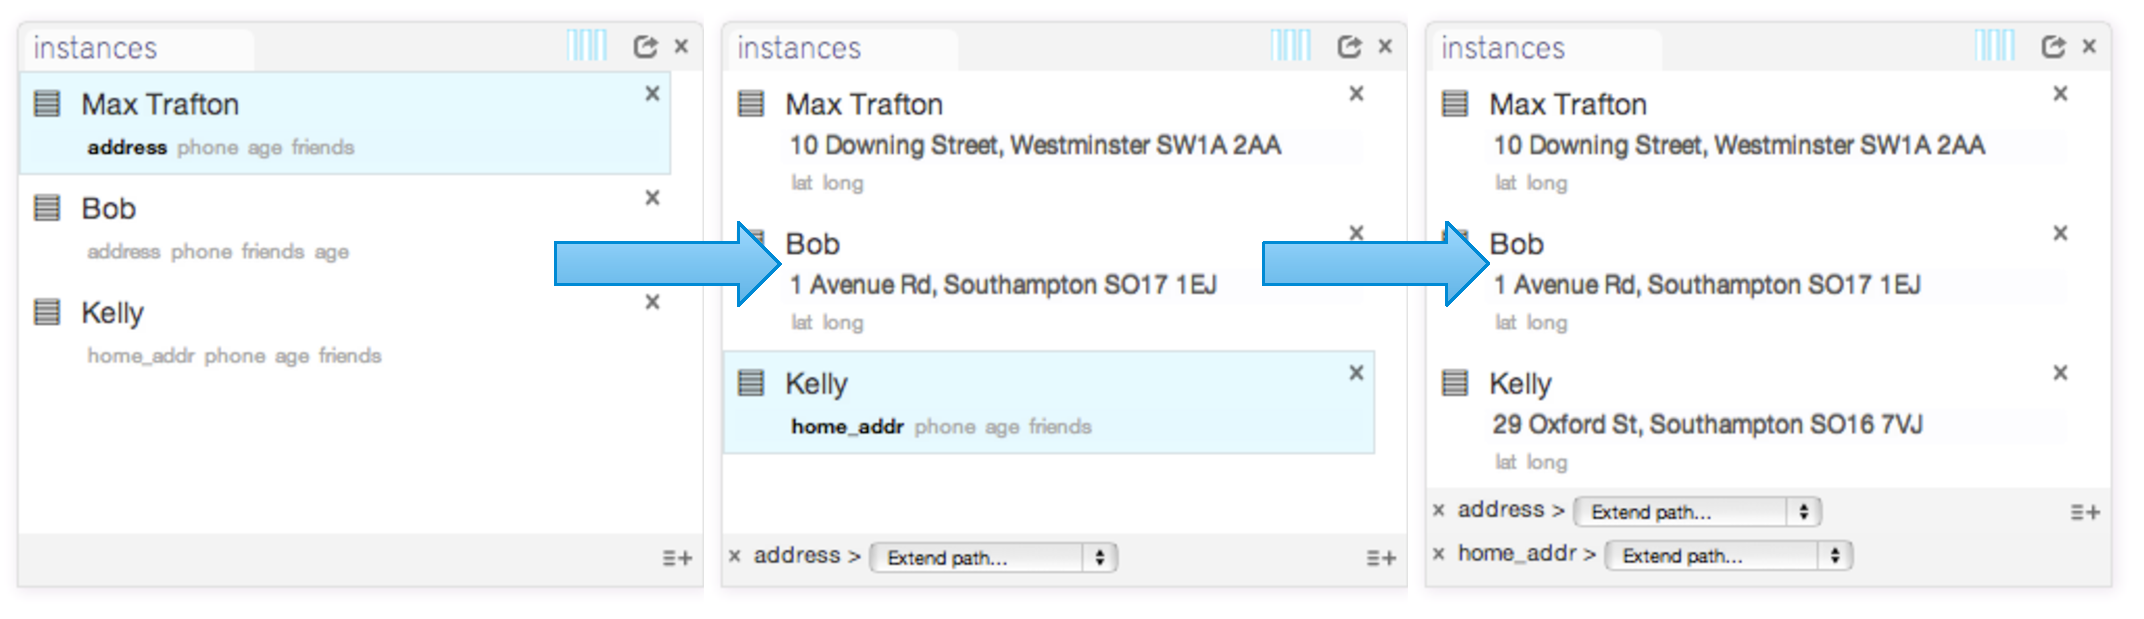
\includegraphics[width=8.5cm]{img/multipathing}
\caption{To see properties, users click on the name of the property. When instances do not have a particular property, additional property names can be added.}
\label{fig:multipathing}
\end{center}
\end{figure}

Typically, users are interested in viewing and comparing the \emph{properties} of instances; for example, a user might be keen to examine a product's price, rating, manufacturer and so on.  An instance's properties are displayed beneath it; selecting a property creates a \emph{path selection}, which dereferences all of the instances in a group that contain the selected property and displays their corresponding values.  For example, when a user selects the \emph{manufacturer} property for a product, all products in the same group with a manufacturer property will be dereferenced, causing the manufactueres to be displayed alongside their corresponding products.  When such a path selection is applied, the properties displayed are updated to be the set of properties of the \emph{terminating value of the path}, so that this value can be dereferenced further.  For example, once selecting a manufacturer, a user may want to know the product's manufacturer's reputation and selects their ``reputation score'' property, causing the previous path selection to be extended. This process is illustrated in Figure \ref{fig:multipathing}.

When instances cannot be dereferenced by the chosen path selection, an additional path selection can be created. As with the first path selection, it causes all matching instances to be dereferenced.  Each group can carry an arbitrary number of path selections, and each path selection can be extended continually by selecting successive properties of values. This achieves the ability to \emph{link slide} as introduced by Parallax~\cite{parallax}, but across sets of heterogeneous items by supporting multiple parallel dereferenced paths simultaneously.  

Multiple selection group-dereferencing results in two effects: 

\begin{enumerate}
\item Clicking on a property dereferences all corresponding values makes it easy to quickly compare all instances that have the same structure.  Although we were concerned that users might be surprised that path selection applied to all objects within each group in parallel, users adapted very quickly and used this functionality to save them time.   

\item Supporting dereferencing along different paths \emph{by structure} allows instances with different property names, and even sub-structures to be quickly consolidated by separate dereferencing, thereby effectively coping with terminological and structural heterogeneity.
\end{enumerate}

\subsubsection{Coreference consolidation: Drag-and-Drop Same-as}

\begin{figure}[htbp]
\begin{center}
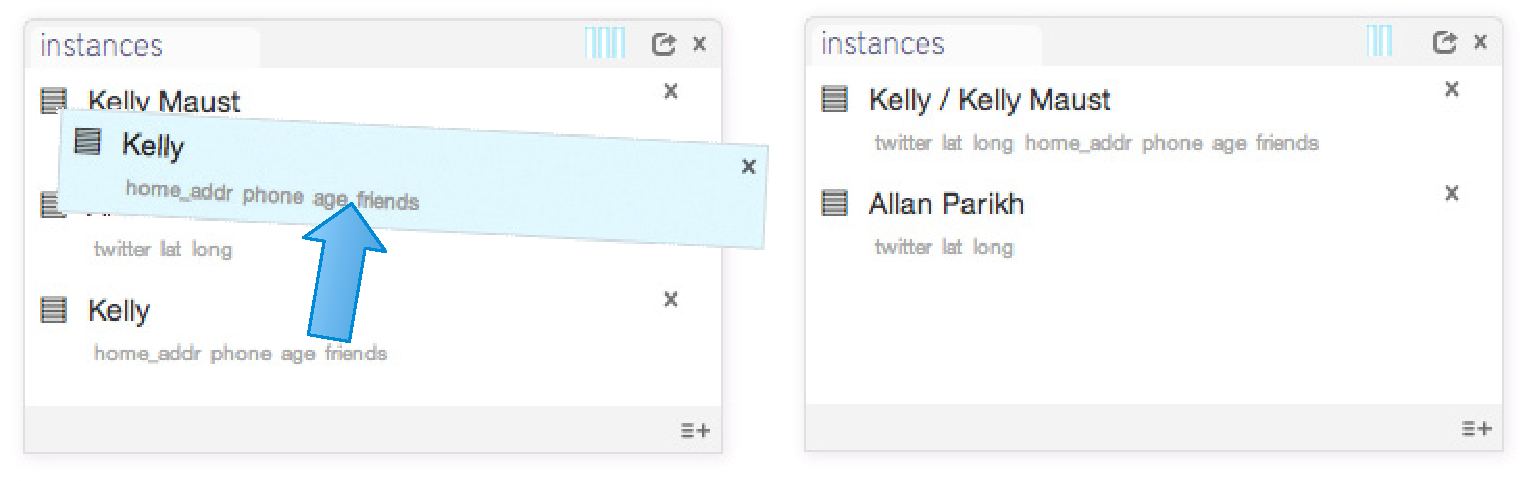
\includegraphics[width=8.5cm]{img/sameas}
\caption{\emph{Coreference consolidation with drag-and-drop Same-As} - When two instances represent the same entity, users can drag one on top of the other, and they are combined - effectively displaying the union of properties of both source entities. This can be un-done by deleting the Same-As relationship in the view in the lower-left corner of the workspace.}
\label{fig:sameas}
\end{center}
\end{figure}

A major challenge with integration from multiple sources is coreference consolidation, or combining representations that co-refer to the same entity into one.  For example, consolidating one's friends from Facebook, Google+, and LinkedIn, one might quickly want to de-duplicate and combine friends that use multiple services so that they each have one representation.

Although we considered a way to do this automatically, PS.2 revealed no way to reliably identify co-referring instances; due to a lack of standard URIs across social networks, identifiers used by each network were system-specific and inconsistent. Thus, we sought to make instead make it user-driven, and easy to do manually.  

To remain consistent with the drag-and-drop interactions used throughout the interface, we introduced the ability to simply drag one instance on top of another to specify that two things should be combined.  This action also caused the \emph{same-as display} in the lower left of the screen to display this new combination relationship.  The display also acted as a mechanism to delete/undo combinations, which reverted representations of instances back to their original, separate forms. An illustration of this interaction is provided in Figure \ref{fig:sameas}. Although general, this can be tedious for groups of items.  Thus, to support more efficient combination, we extended this to allow entire groups to be dropped on other groups.  When this is done, DataPalette attempts to identify matching pairs among items in the dragged and target groups by comparing each pairs' labels.  Only exact matches (modulo white space/underscores) are considered matches and automatically combined.  The rest are added to the target group as distinct elements, and may be explicitly combined by hand.  We are considering more sophisticated / less fragile approaches to matching in the future, which would make the system assistive. 

By making such consolidation user-driven, we gave the user freedom to combine things when it suited him or her. As we saw in the system evaluation, while in certain circumstances users preferred combining representations, in others people preferred to keep things separate.  Thus, user-initiated consolidation afforded an additional flexibility that was ultimately deemed beneficial.

\subsubsection{Enumerated-type value consolidation}
Related to the concept of co-reference, PS.2 revealed that enumerated values of properties were often inconsistent, e.g. ``Casual dining'' vs ``Relaxed'' for a restaurant's ``atmosphere'' property. To reconcile and consolidate corresponding values from different  datasources, we extended the drag and drop support of co-reference combination to also allow users to drag and drop to combine enumerated literal values as well.  

\subsubsection{``Do What I Mean'' Visualisation}

To make it easier for people to quickly visually compare aspects of instances, we created a charting tool and integrated a mapping feature.  To make these tools suitable for fast use, e.g. data exploration, we designed these tools to automatically configure display parameters instances or groups of were dropped on them, rather than making users manually specify them. In the current prototype, the DWIM behaviour of the chart automatically sets whether the plot is a histogram representation (counts of values) or numeric value display based upon the types of the dereferenced values being plotted; values that are non-numeric are counted, while numeric values are displayed.    Similarly, the map was made to detect address strings and latitude/longitude pairs, geocoding them where appropriate, and determining the optimal bounding box to display all items at maximum zoom.

\subsubsection{Model-based brushing}
Since it can get confusing having a single instance represented across several groups, we provided \emph{universal brushing} across the interface; hovering over any representation of any instance (an instance block, a map marker or a histogram bar), causes all other visible representations of that instance to lightly glow, so that the user can quickly identify all the places that a single instance is represented

% Data sources were represented as collapsible panels in a sidebar on the left of the workspace, from which instances or entire data sources could be ``pulled off'' onto the workspace.  Figure \ref{fig:workspace} displays the entire UI overview.

%% it would be nice if we had space to summarize but i fear we don't

%% \subsection{Summary of interaction capabilities}
%% \begin{itemize}
%% \item \emph{Group multi-path value selection} - Selecting any of the %% properties of an instance in a group (window) causes all of the rest %% of the instances that have that property in that group to be %% dereferenced along the same property, displaying the resulting value %% underneath the instance label.  Selecting a further property of the %% resulting value further dereferences this value.
%% \item \emph{Drag-and-drop coreference / value combination} - In order %% to specify that two instances correspond to the same entity, they can %% be simly dragged together
%% \item \emph{Group-based Drag-and-drop matching} - In order to specify %% that two instances correspond to the same entity, they can be simly %% dragged together
%% \item \emph{Universal model-based brushing} -
%% \end{itemize}

\section{Evaluation}

In order to determine whether the interaction affordances introduced in DataPalette (henceforth DP) allow users to perform serendipitous data mixing on real data feeds by end-users, we devised a within-subjects A-B trial lab study which we describe next.

\subsection{Methodology}

We first describe our methodology, starting with the three hypotheses we set out to test:
%These hypothesis pertain to the usability of DP by end-users (h1), whether DP achieves its stated goal of enabling end-users to integrate data (h2), and finally if it has an effect on task performance (h3) - either in how well people perform a task, how quickly they perform it, or if it reduces task effort, as follows:


% heather: instead of these low-level hypotheses, i've made higher level ones that we can explicitly address in the disucssion section - the more hypotheses we have, the more we have to come back to them; since we're short on space we might as well keep it simple!

%% Interaction-method specific hypotheses
%% \begin{itemize}
%% 	\item h1.1 - Do people understanding the problem of %% co-reference, and the need to reconcile coreference problems?
%% 	\item h1.2. Does the ability to do drag + drop combination for %% co-reference reconciliation effectively solve this problem?
%% 	\item h2.1- Do people understand the problem of structural %% differences in data?
%% 	\item h2.2 - Does multipath selection let people effectively %% deal with this -- and work with collections of heterogeneous items?
%% \end{itemize}
%% Are these interaction methods sufficient to perform common tasks %% involving heterogeneous data sources?  Does supporting these simple %% techniques facilitate task completion?

\begin{description}
\item [h1. Usability -] People understand how to use DP.
\item [h2. Data Integration -] People can effectively mix heterogeneous data with DP.
\item [h3. Task completion -] Use of DP improves people's ability to perform the task.
\end{description}

\subsubsection{Study and task design}
To test these hypotheses, we designed a within-subjects lab-based A-B study in which participants were asked to perform two predefined tasks in separate timed trials, once with the DP interface (``condition A'') and once with a baseline interface (``condition B'' which we describe below).  We used upon the within-subjects A-B format in order to make both quantitative measurements about an individual's performance with DP (relative to baseline), but also to make qualitative observations of the processes used by each participant as they solved each task.  Each task was paired with one of two datasets, depending on condition, so that we could evaluate whether the participant's performance of completing a task differed with different datasets.  Conditions and interface order were fully counterbalanced among participants to eliminate ordering and task bias.  

% why? why were these tasks selected? can we drop in the phrase ``multi-dimensional subjective choice task'' and refer back to PS.1 to justify the choice of tasks?
We based our two tasks on choosing a university and picking a restaurant for a large social event, because in PS.1 the majority of people stated that they had used multiple websites for these tasks.  We used different two different variables for both tasks, where the restaurant was located (Glasgow and Cambridge) and which subject people choose (sport science and history).  The cities Glasgow and Cambridge were chosen because they are not geographically close to the participants, they are two heavily populated areas that have a choice of restaurants, and they contained detail data about the same restaurants on various review sites.  When deciding on which cities to use, we found that different areas favoured different review websites and places such as Hull had sets of disjoint sets of restaurant reviews.  We selected the top restaurants for on Tripadvisor and Yelp, because they were the top two websites people quoted for comparing reviews when travelling.  We selected the two university courses at random from a list taken form the complete university guide\footnote{}, and selected the top six university for that subject because they provide a realistic shortlist and are comparable in terms of rankings and properties.   We selected a shortlist of six because it is typical for users to narrow down their options to a limited selection before analysing the details of their final choice.

\subsubsection{Task preparation}
% how data was prepared for each of the tasks; exactly how the A condition was done (full screen DP in a web browser, no outside access to apps),  B condition and why
In order to prepare the data for our tasks, we identified websites that people commonly used for selecting universities and restaurants.  Once we had compiled the list of websites, we select the top most used six for each task.  We selected six because it enable us to scope our study, we found through two pilot studies that six data sources provided a sufficient challenge for users to explore the data and required them to use DP's main features.  We manually collected the data from the nine selected websites into jason files, and converted them to Microsoft Excel worksheets (which 40\% of the participants in PS.1 said that had previously used to compare data).

% why was the B condition set up this way? What did we seek to achieve?
The control (B) conditions were in a prepared Mac comprised of a web browser pre-loaded with a page with links to four live web sites, and an open instance of Excel with a workbook open containing spreadsheet versions of the same data as were loaded into DP for the A condition versions of the same tasks.  Other Office applications were also available for use and participants were allowed to visit other sites than the pre-specified ones.  The purpose of this condition was to understand how people using standard desktop office software.

\subsection{Data Collection and Analysis}
Each study was overseen by a facilitator and an observer:  the role of the facilitator was to explain the study's protocol to the participant and to answer any questions; and the role of the observer was to observe without interacting with the user, and to take notes.  Both the facilitator and observer were trained on the purpose of the study, their role and how they could and couldn't influence the study.   Explicitly both the facilitator and observer where trained in identifying processes that people used during a task, so that they could thematically categorise them.  Initially, we identified the following themes: organisation of data, eliminating candidates, co-referencing, and visualisations. The studies were run over 4 days.  At the end of each day the facilitators and observers met to discuss the studies' data and to revisit protocols, if necessary.  During the lab study, we recorded the audio and the participant's actions on screen. We asked the participants to follow a \emph{think-aloud} protocol as they worked, so that we could understand the reasoning behind their actions.  At the end of the study, the participant completed an exit survey.

We planned to analyse the qualitative and quantitative data using thematic and statistic analysis, respectively.  In order to carry out our data analysis, we used the recorded transcripts to populate a spreadsheet summarising the quantitative metrics (see Table \ref{tbl:data} for specific fields).  In our study, we aimed to identify process and strategies people used to complete their tasks, so that we could evaluate the effectiveness of DP's interface when aligning heterogeneous data for organisational tasks.  We also categorised people's views voiced during the study and in their exit survey pertaining to DP's usability and interface, and clustered them to evaluate common feedback.

\subsection{Participant Recruitment}
We recruited participants through adverts posted near the University campus and e-mails to student mailing lists.  We screened participants to be at least 18 years of age, but did not filter or preferentially select participants based on any other criteria.  We took the first 20 that signed up and that successfully specified time slots that were available.   As described below in results, we ended up getting a large number of international students, who had varying proficiency in English.  Since all such participants had passed the requisite proficiency tests to enrol at University, we did not think this would substantially impact results.  Participants were offered a small gift certificate from an online retailer for their time. 

\subsection{Experimental Setup}
The participants were given a standard desktop PC running MacOS X on a 22-inch monitor with a standard keyboard and mouse.  During the studies the Excel workbook and DP were initially set to full screen.  Each participant was asked to complete two tasks, one A and one B condition.  Each participant was given a maximum of 10 minutes to complete a task, but were told that if they finished earlier they could tell us and move on to the next condition.  In order to select which tasks the participant was given, we used a latin square to permutate the tasks and conditions.  In order to train the user on how to use our interface, they viewed a five-minute DataPalette tutorial video introducing its basic functionality, how to use histograms and maps, and linking instances.

%Each task had an A and B condition.  The A condition, the participant could only use DataPalette to make their decision; and in the B condition the participant was given the choice to using any websites they desired and or workbook in Microsoft Excel containing the data taken from the data sources to make their choice on individual spreadsheets.

%Each study consisted of two tasks, one A and one B condition.  Each participant was given 10 minutes to complete a task.  In order to select which tasks the participant was given, we used a latin square to permutate the tasks and conditions.  In order to train the user on how to use our interface, they viewed a five-minute DataPalette tutorial video introducing its basic functionality, how to use histograms and maps, and linking instances.

\begin{table*}[t]
\begin{center}
\small
\begin{tabular}{|p{4cm}|p{6cm}|p{6cm}|}
\hline
Task	 &Choices	&Data Sources\\
\hline
1) Three universities they would apply to study Sport Science & Universities: 1) Loughborough,  2) Durham,  3) Exeter, 4) Edinburgh, 5) Birmingham, and 6) Bath & http://www.thecompleteuniversityguide.co.uk/, http://www.ucas.ac.uk/, http://unistats.direct.gov.uk/, http://www.timeshighereducation.co.uk/world-university-rankings/ \\
\hline
2) Three universities they would apply to study History & Universities: 1) Cambridge, 2) London School of Economics and Political Science, 3) Durham, 4) Oxford, 5) St Andrews, and 6) University College London & http://www.thecompleteuniversityguide.co.uk/, http://www.ucas.ac.uk/, http://unistats.direct.gov.uk/, http://www.timeshighereducation.co.uk/world-university-rankings/ \\
\hline
3) Restaurant they would book for 12 friends in Cambridge&Restaurants : 1) Alimentum, 2) Gardenia Restaurant, 3) The Cambridge Chop House, 4) Al Casbah, 5) Midsummer House Restaurant, and 6) Nando's Restaurant. & www.yelp.co.uk, www.tripadvisor.co.uk, http://ratings.food.gov.uk/, facebook and google plus.\\
\hline
4) Restaurant they would book for 12 friends in Glagow & Restaurants :1) Black Sheep Bistro, 2) Charcoals, 3) Number 16 Family Restaurant, 4) Fanny Trollopes Cafe, 5) Two Fat Ladies At The Buttery, and 6) Sapori D'Italia. & www.yelp.co.uk, www.tripadvisor.co.uk, http://ratings.food.gov.uk/, facebook and google plus.\\
\hline
\end{tabular}
\end{center}
\caption{Tasks, choices and data sources} \label{tab:studyfactors}
\normalsize
\end{table*}%



%\subsection{Data Analysis} 

%% TODO - emax doesn't like this paragraph - kill it? 
%During the data collection we collated a spreadsheet summarising the participant's gender, typical daily computer usage, the tasks allocated and basic actions performed during the task.  After we had collected the study's data, we performed our data analysis. 

%% TODO look further into types of data analysis....

\section{Results}

Twenty-six (26) participants responded, from which we selected the first 20.  Ten participants were female.  All of the participants spoke English, but 12 of them were non-native English speakers.  Seven were non-students, comprising University staff and alumni; out of the remaining 13, eight studied computer science and 5 studied other subjects.   On average, each study took 40 mins to complete.  The information in Table \ref{tbl:data} summarises the metrics that were captured of the trials for each participant. We analyse this data next.

\begin{table*}[htdp]
\small
\begin{center}
\begin{tabular}{|r|p{0.3cm}|p{0.3cm}|p{0.3cm}|p{0.3cm}|p{0.3cm}|p{0.3cm}|p{0.3cm}|p{0.3cm}|p{0.3cm}|p{0.3cm}|p{0.3cm}|p{0.3cm}|p{0.3cm}|p{0.3cm}|p{0.3cm}|p{0.3cm}|p{0.3cm}|p{0.3cm}|p{0.3cm}|p{0.3cm}|}
\hline
Participants & 1 &2&3&4&5&6&7&8&9&10&11&12&13&14&15&16&17&18&19&20\\
\hline\hline
gender&f&m&f&f&f&f&f&m&f&f&m&f&m&f&m&m&m&m&m&m\\
A condition first task &y&y&y&n&n&y&n&n&y&y&n&n&y&y&n&n&n&n&n&n\\
\hline\hline
A Condition: task &4&2&3&4&3&&2&1&4&1&4&1&3&2&3&2&1&4&3&2\\
paper used&n&n&n&n&n&n&y&n&y&y&n&y&n&n&y&n&n&n&n&n\\
charts used &1&2&2&0&2&4&5&0&0&0&2&3&2&0&0&0&3&3&4&1\\
maps used &1&1&2&2&2&1&1&0&1&0&1&1&2&1&0&1&0&0&2&1\\ 
same as used &4&3&3&6&0&2&0&2&1&0&6&5&6&2&7&0&6&7&7&7\\
\# data sources used &4&3&4&4&4&3&4&3&4&4&3&3&5&4&5&4&4&5&5&4\\
chosen restaurant/uni &4.1&2.4&3.5&4.3&3.3&&2.4&1.4&4.2&1.6, \newline 1.3, \newline 1.2& 4.2& 1.4, \newline 1.5, \newline 1.3& 3.2& 2.1, \newline 2.3, \newline 2.6& 3.5, \newline 3.3&2.6, \newline 2.3, \newline 2.5&1.6, \newline 1.5, \newline 1.3&4.1&3.3&2.4, \newline 2.5, \newline 2.6\\
\# factors in choice &-&-&-&-&-&-&-&-&-&-&-&-&-&-&-&-&-&-&-&-\\
\hline\hline
 B Condition:task &3&&4&3&4&2&1&2&2&3&2&3&1&4&1&4&2&2&1&3\\
 paper used &n&n&n&n&n&n&y&n&y&y&n&y&n&y&y&n&n&y&n&n\\
 spreadsheet/website&&&&&&&&&&&&&&&&&&&&\\
 number of spreadsheets used&5/5&4/4&2/5&1.5&2/5&5/5&4/4&2/4&3/4&&2/4&4/5&2/4&4/5&2/4&2/5&4/4&4/4&0&5/5\\
 number of websites used&1&1&4&3&3&0&2&3&2&&1&2&3&1&2&3&2&0&4&0\\
 chosen restaurant/uni&3.5&&4.2&3.3&4.3&2.1&1.4, \newline 1.2, \newline 1.6&2.1&2.3, \newline 2.6, \newline 2.5&3.5&2.2, \newline 2.3, \newline 2.6&3.5&1.1&4.1&1.6&4.2&2.6, \newline 2.3, \newline 2.5&2.3, \newline 2.5, \newline 2.6&1.1, \newline 1.3,  \newline 1.4&3.5\\
 \# factors in choice &-&-&-&-&-&-&-&-&-&-&-&-&-&-&-&-&-&-&-&-\\
 \hline
\end{tabular}
\end{center}
\caption{Participants data.} \label{tbl:data}
\normalsize
\end{table*}

\subsection{Task performance}

The following four sections describes the metrics we used to measure task performance.
%We used three metrics to measure task performance: time to completion; the number of factors used in the choice; and the number of candidates evaluated.

\subsubsection{Efficiency: Time taken}
Participants spent an average of 8.9 minutes performing the tasks, with our interface, condition A, taking slightly less time ($M=8.7$min, $SD=1.79$) per trial than condition B ($M=9.0$min; $SD=1.44$).  An ANOVA test of time taken by interface condition blocking by participant did not find interface use a significant predictor of task completion time (shown in Figure \ref{fig:time}).  Although across trials, the restaurant selection task took on average slightly less time ($M=8.8$min,$SD=1.58$) than the university trials ($M=8.9$min,$SD=1.66$), the aforementioned ANOVA test found task type to not be a significant predictor.

\subsubsection{Thoroughness: Factors weighed in final choice}
The second metric was the number of factors the participant considered in making their final choice. To determine this, we asked participants explain precisely why they made their choice, and matched their justifications to properties in the data.  This analysis revealed a significant effect of interface on number of factors weighed ($F(1,19)=3.95; p<0.10$); participants in the DP condition listed an average of 5.5 choices in their decision ($SD=1.7$) versus 4 ($SD=1.73$) in the standard condition.

\subsubsection{Diversity: Data sources consulted}
The third metric we used to gauge how well the participant performed their tasks is the number of different data sources the participant consulted during the trial. In this metric, participants used an average of 88\% of data sources provided in the DP case, compared to 80\% in the standard interface, although an ANOVA test blocking on participant demonstrated that interface choice only approached significance in predicting the number of sources consulted ($F(1,19)=0.04$ $p\approx0.10$).

\subsubsection{Effort: External cognition}
Although we did not have an explicit measure of effort for this experiment (such as NASA's TLX \cite{tlx}) the use of paper notes provided an indicator of how much participants had to keep track of during the study.  We found that participants took notes less on average (25\%) with the DP interface than the standard interface (35\%), a difference which approached significance in an ANOVA blocked by participant ($F(1,19)= 8.22; p\approx0.10$).

\subsubsection{Candidate selection}

\begin{figure}[htb]
\begin{center}
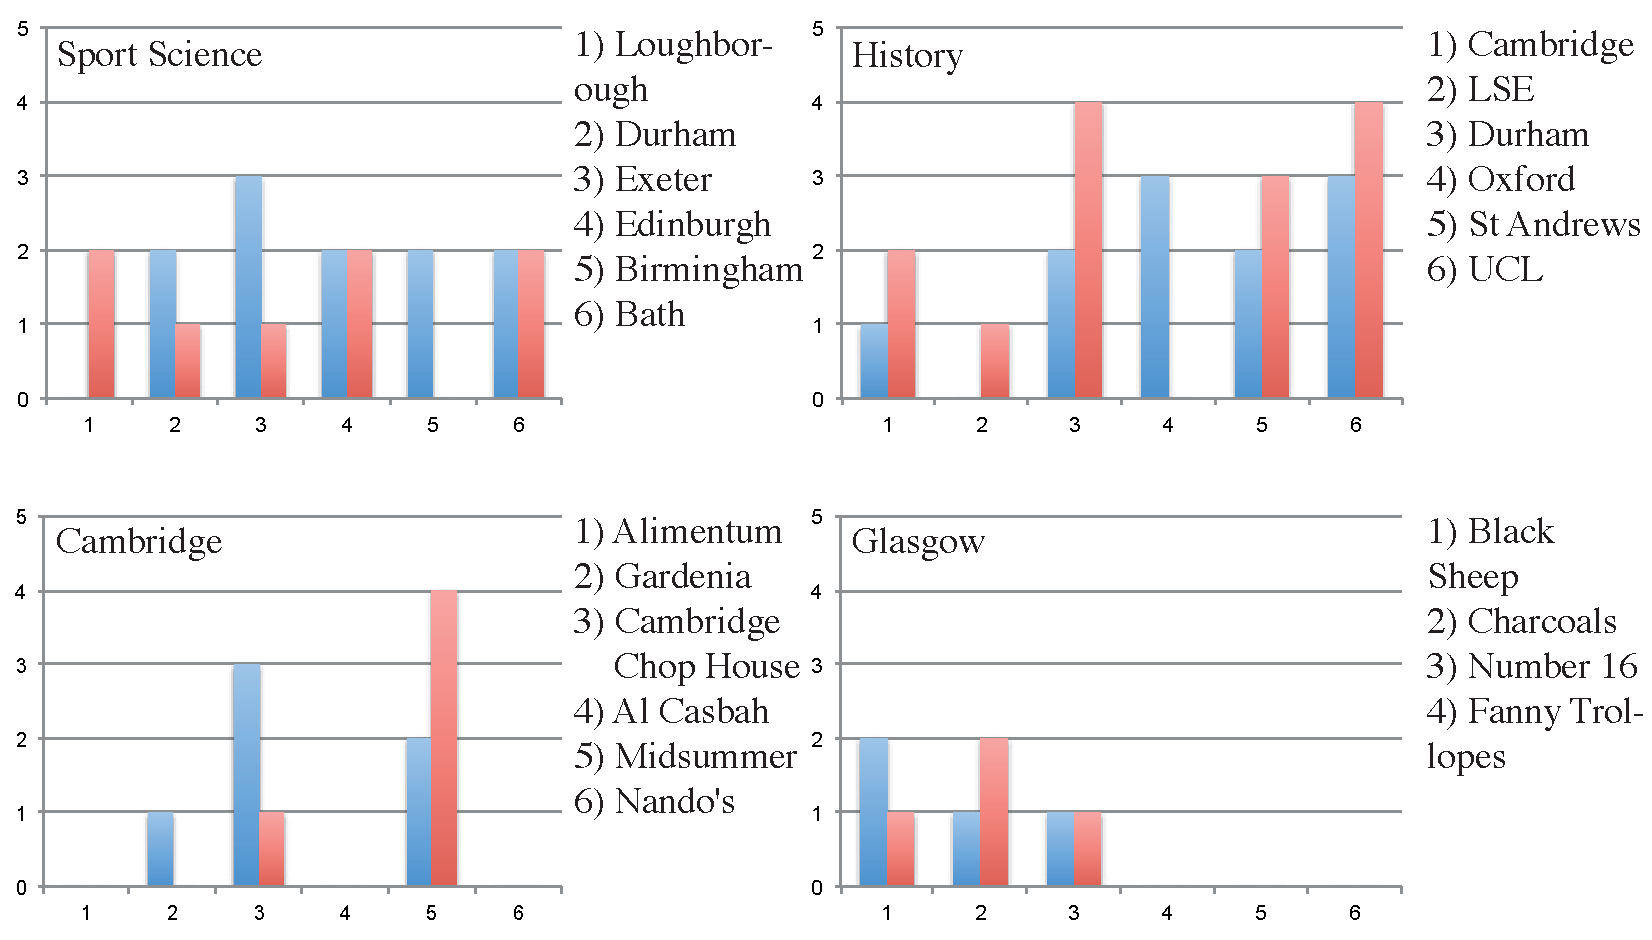
\includegraphics[width=8.5cm]{img/results}
\caption{\emph{Choice picks per participant trial} - Histogram of number of times each restaurant/university was chosen in DP interface (A condition) in blue/left bars, compared to the Excel/website (B condition) in red/to the right.}
\label{fig:chosen_results}
\end{center}
\end{figure}

Since the tasks were subjective-choice, we could not evaluate the 'correctness' of people's answers.  However, to determine whether there was a difference in variability of answers between interface conditions, we plotted their choice on a histogram for each trial, per task and dataset for both conditions, visible in Figure \ref{fig:chosen_results}.  As can be seen there is considerable variability and no discernible difference in variability between conditions.  

\subsection{Strategies: Successive Elimination vs Tallying}
As described in later this section, we noticed several different strategies people used to evaluate each candidate selection. One common strategy was \emph{successive elimination} - to look at a single dimension at a time, starting with the most important, ruling out candidates that did not meet the required minimum for that value.  However, when there is no clear ``most important'' aspect, this  ``greedy-style'' can result in suboptimal decisions.  Another strategy, which we called \emph{tallying the pros and cons}, kept all candidates around, and counted up the advantages and disadvantages of each, potentially weighing each factor by its perceived importance.  This strategy is less vulnerable to getting stuck in local maxima than the former.

To understand whether the interface influenced choice of strategy, we measured the number of candidates that the participant considered \emph{at final result}.  This we found was a strong marker for use of each strategy; people using the successive elimination strategy arrived with only 1-2 candidates at decision time, while those that tallied still maintained the entire starting set.  

We found that the use of DP strongly influenced people to keep all candidates around, while participants in the B condition eliminated choices early.  An ANOVA test demonstrated a significant effect between condition and number of candidates maintained ($F(1,19)=5.323; p<0.05$); a post-hoc Tukey HSD test confirmed that  the number of candidates used in the final choice for participants in the A condition ($M=5.85;SD=0.45$) differed significantly from the B condition ($M=4.95; SD=2.26$).

\subsection{Use of Data Integration Features}

To determine whether participants used the data integration features of DP, we looked at use of the \emph{multipath selection} and \emph{Same-As} features of the system.   Pertaining to path selection, all participants readily used the path selection process to select values.   Five participants (25\%) deliberately used multipath selection, defined as selecting more than one active path per group at the same time to display common values across heterogeneous items. (We did not count accidental use of multipath, such as happened a few times when a participant had an already active path and wanted to switch to a separate path accidentally).

Participants used the drag-and-drop \emph{Same-As} capability extensively. Sixteen (80\%) used \emph{Same-As} as least once; among these participants, they used \emph{Same-As} an average of 4.6 times per trial. We counted a single ``use'' as a single drag-and-drop of an individual item, or a drag-and-drop operation of an entire group onto another.  (We did not differentiate enumerated value consolidation from entity consolidation, as these operations were not discernably different from the interface perspective.)

% we examined use on performance but nothing significant was found :/

\subsection{Use of Visualisation Features}
To determine to what extent visualisation tools were used in condition A, 13 (65\%) used charting tools at least once, while a majority (15, 75\%) used the map.  Determining the impact these had on performance, we performed a multiple regression on time taken with the number of uses of charting and mapping as variables.   We found significant effects of both charting and mapping variables on time taken, ($R^2_{adj} = 0.04; F(2,17)=3.79; p<0.05$), with coefficients ($Y_0=8.91;\beta_{charts}=0.49;\beta_{maps}=-1.05$) demonstrating that charting positively influenced time taken, while the use of maps led to shorter times.

\subsection{Condition B - Results and Observations}
In the B conditions, participants were given the option of using websites and or a spreadsheet to make their choice.  For B trials, we measured the fraction of the trial time spent in Excel versus looking at the sites in a 5-value range (0,25,50,75,100\%).  Six individuals used Excel entirely (100\%) without consulting the web sites, while one avoided Excel entirely; most fell somewhere in between, with median use at 75\%.   When asked to explain their choice of tool post-hoc, participants who used Excel explained that it saved them time over individually searching and consolidating information from the websites (10 participants).  Participants used websites when they needed to know more than what was provided in the spreadsheets (8 participants), when they mistrusted the information in them (1 participant), or if they were not familiar with Excel (1 participant).

Participants ran into a number of difficulties with the spreadsheet interface. Participants struggled with looking up values across different worksheets (data sources).  Some attempted to collate all data onto a single sheet, so that they could compare the values all at once; however, this approach was often error prone.  For example, two participants did not notice that the rows in two sheets were in different order, causing their pasted values to be incorrectly mapped.  Four participants struggled with sorting columns, and only 1 attempted charting (p7).  Although she attempted to plot multiple factors simultaneously, Excel's charting features caused her considerable difficulty and she eventually resorted at creating multiple simple bar-charts instead.

While most participants only made minor formatting and column sizing changes to the worksheets to facilitate reading and interpretation,  four made extensive edits to the sheets to help them ``think through'' the task in various ways.  These uses of Excel for external cognition ranged from the collation behaviour just described to tallying annotations, to colour-coding cells to allow easy identification of  ``pros'' and ``cons''; ``I can't deal with so many textual values; I need colours to help me see'' (p6). Another user calculated their own weighted metric of which university to choose by averaging different metrics supplied by the data sources and filling in their own chosen weights.  

%%  was use of pen and paper to collate the values, which was often faster and resulted in less observed frustration. While the majority of users did not attempt anything complex with Excel (in fact only one user used charts), there was some advanced use of Excel observed.

%% todo - look up to make sure it was really p7 here 
Various difficulties were also encountered with use of the websites. There was significant confusion over various attributes, especially in the University selection task.  For example, p15 could not tell how the teaching score from the Times Higher Education was calculated, in order to assess its relative importance.  Several participants had difficulty finding information they needed because of inconsistencies in site layout, especially finding course requirements, information that ``should be obvious''.  Similar issues were encountered with finding information in the restaurant condition; p7 said ``I wish they would put Cuisine Type in the same place for every restaurant - important information!'' Similarly, participants found it difficult to visualise the locations of restaurants in cities that they were not familiar, and could not find a way to easily map them. Overall, the users that spent the most time using websites exhibited significant frustration attempting to locate and compare different criteria (such as course entry requirements, or restaurant locations), and often ended up swapping back to using the supplied spreadsheets.


% Notably, a number of users admittedly introduced their own bias into the choices in both A and B conditions: ``I prefer Indian food, so I will choose the Indian restaurant'', and one participant spent time on Google Maps looking at the routes to each restaurant, and eliminating those that required bus transfers (the protocol did not mention routing/transfers at all).

\subsection{Survey Results}


\begin{figure}[tbp]
\begin{center}
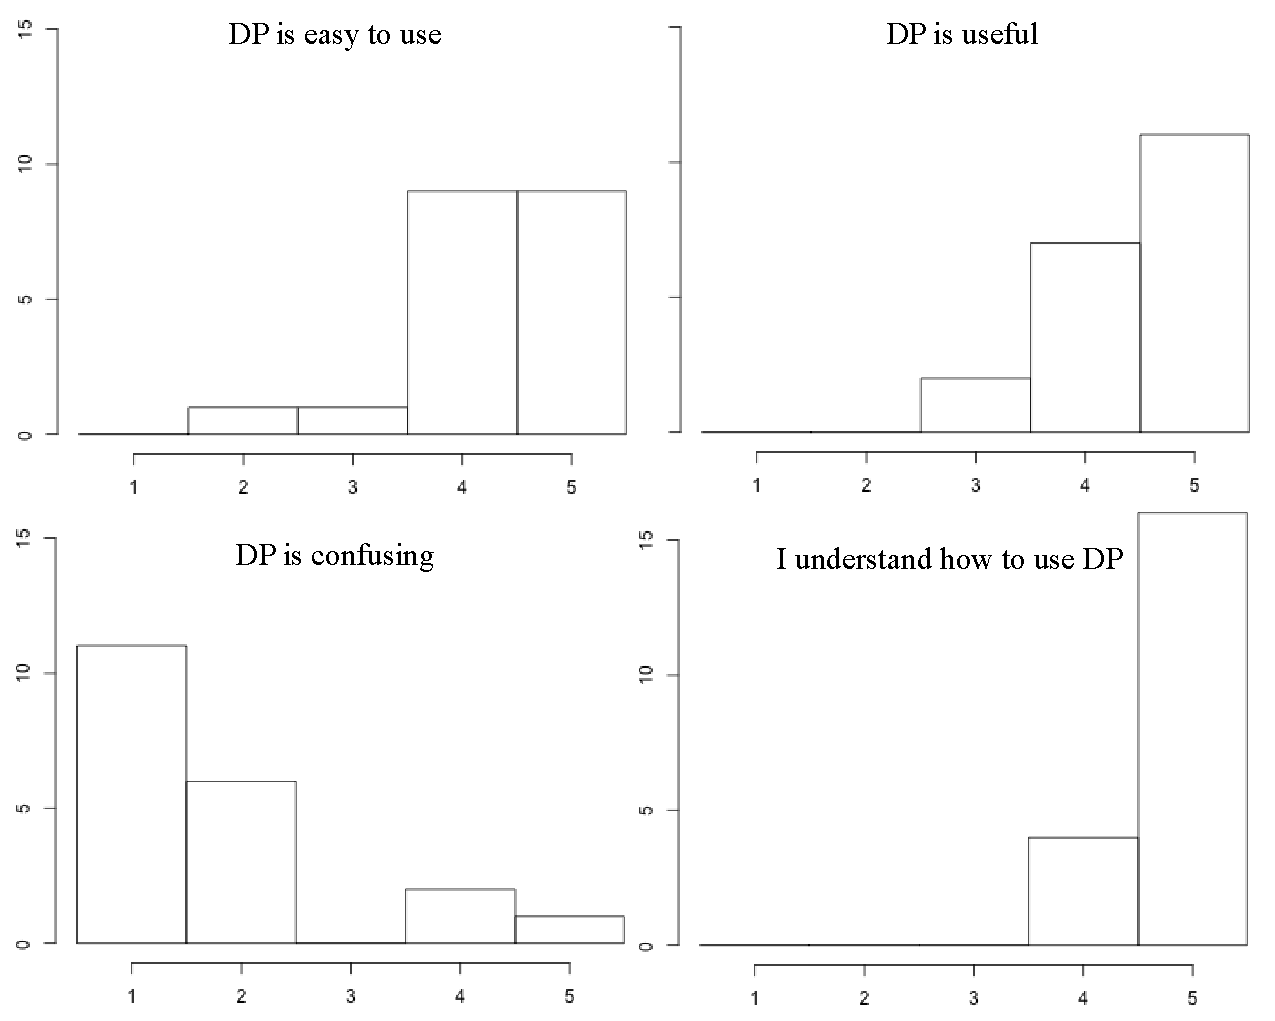
\includegraphics[width=7.5cm]{img/survey}
\caption{\emph{Survey results} - Answers to questions on a 5-point Likert scale, from 1-\emph{strongly disagree} to 5-\emph{strongly agree}.}
\label{fig:survey}
\end{center}
\end{figure}

When asked to rate the DP interface, all participants responded that they felt they understood the system, with sixteen (80\%) responding that they agreed \emph{very strongly}.  Eighteen (90\%) reported that they thought  DP was \emph{easy}, as well as \emph{useful}, with one person being neutral on each.  On the statement ``DP is confusing'',  11 strongly disagreed, 6 disagreed, and 3 agreed.  Revisiting the time trials, we discovered that the 3 participants who rated DP as confusing completed the trials statistically significantly slower than the rest of the group. Survey results were visualised in Figure \ref{fig:survey}.

%+What did people think about it? 
% Usefulness,Ease,Confusion,etc

In the exit survey, the users noted that they would use an interface like DataPalette in the future, for finding a property to rent/buy, choosing a job and purchasing electronic devices.  However, one participant said that they would not use it for things like deciding on a restaurant because ``it would cheapen the experience'' by removing the element of spontaneity of choice, but would use it for making more important decisions.  In order to improve our solutions the participants suggested making the origin of the information clearer, particularly when combining multiple data sources. The participants also requested the ability to sort instances, as well as explanations of ratings and scoring systems (however some of these are not even transparent on websites). Participants also requested standard features not present in our prototype, such as window management options (specifically, arranging and minimising windows), and the ability to undo operations.

\section{Discussion and Limitations}

In this section, we first re-visit our study hypotheses introduced in Methodology, using observations from results to support views on each.  We follow this with a discussion of limitations regarding the design of the interface, the state of the prototype, and the design and execution of the study.  Finally, we discuss our current and follow-on plans for continuing this line of research.

\subsection{Revisiting the hypotheses: Does DataPalette facilitate serendipitous data integration?}

We set out to answer three different questions with the DataPalette study. The first concerned whether people understood and could use the system (h1), whether the system enabled people to mix and integrate heterogeneous data (h2), and whether the interface facilitated task completion (h3).  Using real data obtained from typical data sources identified during our prestudy (PS.1), we tested the DP prototype and its integration interaction mechanisms with ``real'' users, who were students, staff and alumni of our University who had varying backgrounds and levels of expertise with computers.

We find substantial support for h1. All participants reported that they understood the tool, and that it was easy to use.   All participants managed to use the interface to view, organize and collate data without running into major roadblocks or confusion, and all effectively were able to compare multiple attributes of heterogeneous data items directly.  More than half of the participants used DP's visualisation features (charting or map -- often several times during the trial -- suggesting that these features were useful and usable as well.  

Additional evidence that participant had a solid understanding of the system was their feedback, specifically feature requests and desired capabilities.  Several participants requested search functionality, sort and filter functionality, the ability to display multiple properties for a single instance simultaneously, and visualise multiple attributes in a 2 or 3-dimensional visualisation.  Perhaps the most interesting suggestion was also the most common -- the ability to selectively view the provenance of information after instances have been combined.  For example, after his trial, P15 said:

\begin{quote}
Properties are tricky. Sometimes you don’t care [which data source] a property is from, like ``address'' or ``phone number'' - for these the way it’s done now is fine. But in some cases you need context of where the properties come from in order to know what it really means - like for ``rating'', it makes a big difference whether you’re talking about ``Yelp rating'' or some random reviewer's rating.  You also don’t know what typical ratings are, whether 5 stars are much better than 4, etc.
\end{quote}

Pertaining to h2, all participants were able to work with multiple sets of heterogeneous data effectively.  With respect to integration specifically, a majority (80\%) of the particiapnts successfully and deliberately integrated data using drag-and-drop SameAs capabilities.  While single-paths were used, multi-path features were not as widely used, only by 4 participants. We believe that participants may not have realized that creating multiple path selections per group was possible, instead assuming it to be similar to the single ``Current path'' state per window of most file managers. 


Assessing whether DP's improved task performance (h3) was the most difficult to ascertain, given the small sample size of our study and large number of factors influencing each person's performance.  While tasks were completed on average slightly faster than the control interface, these differences were not statistically significant.  However, more data sources seemed to be consulted (we use ``seemed'' carefully because these findings approached significance) during trials with DP over the control interface, which meant that people were looking at more diverse information than the control conditions.  We also found that participants justified their choices with a greater number of factors in DP than the control interface, suggesting that decisions may have been made considering a greater number of factors.  Participants entertained more possibilities for longer in the DP trial, while participants were more prone to eliminate candidates early in the baseline interface.  Finally, people took fewer notes in the DP condition than the baseline, suggesting that there was less need for external cognitive support in DP, which strongly indicates that DP made the task easier to complete.


%% -> discussion and limitations
\subsection{Design Limitations}

In addition to the aforementioned feature requests, we observed a number of ``pain points'' in the design of the interface that we wish to address in the next iteration.  One such pain point was window layout and screen real estate management; participants were prone to opening up a large number of windows, including maps and charts, and found that the screen filled up very quickly.  When the screen got crowded, two problems were observed: people spent a lot of time arranging and moving windows about, and second, people tended to get lost in windows -- ``what was this again?''

\subsection{More Integration Support}

% In the A condition, where participants used DataPalette to complete their tasks, they used it to collate the data on-screen, and compare multiple values directly. About half of the observed users actually used the instance combination feature of DataPalette, with the other half able to successfully make decisions without using it. Those who tried to use it were largely successful, and were able to therefore use the global brush-highlighting to simultaneously compare different statistics. Most users instantly opened up all data sources into individual boxes, in order to determine which sources contained specific statistics. The result of this technique is that the users instantly filled their screen, and ran out of space for plots and maps.

\subsection{Supporting more sophisticated heterogeneity}

Supporting better structural heterogeneity:
   Combining fields
   Splitting fields
   Rearranging fields (British dates American dates)
   
Modelling heterogeneity (?)
   Specificity  
     Education+Jobs vs ``Education'' + ``Jobs'' 

   Unit conversion (kg -> stones)
   Granularity
     Crimes per area

Working with data values

%% \subsection{Better Supporting the Task}

%% - are people more thorough
%% - do they evaluate more sources

%% \subsection{Causing Less Frustration}

%% - Gave up with aspects of the tasks later / not at all
%% - With websites, users gave up on websites and moved on early

%% \subsection{Keeping an Open Mind}

%% - Did users rule out choices less/later
%% - Did that mean they chose "better" options

%% \subsection{What method did people use?}

%% - Processes
%% - Organisation of data/screen
%% - A vs B, how are they different?

% DAN's  qual analysis of processes
%% In order to complete the tasks, the users followed a number of different processes. The most common process followed
%% was {\it collation} of data, either on-screen or on paper. Some users were proficient enough to copy and paste data
%% in the supplied spreadsheets from worksheet to worksheet, while others manually typed data value-by-value across worksheets.
%% Others preferred to collate the data from screen to paper, in order to compare multiple data points. A similar process that
%% some participants followed was to determine which values of a particular statistic were acceptable, and keep a paper tally
%% of these next to the set of choices. They then made their choice based on the value of this tally.

%% Two contrasting approaches that participants followed was to use the data to rule out candidates, or to use the data to
%% directly compare candidates at once. Our pool of participants exhibited both behaviours evenly, however in the condition
%% when using the DataPalette interface, significantly more comparison (and visualisation of values) was performed, with fewer
%% participants using the ``ruling out'' process. A consequence of this was that when asked to justify their choices, users were
%% able to verify their values on-screen immediately, whereas those who had ruled-out had to memorise their reasons, with
%% mixed success  -- many participants had to look through the data sources to re-find the reasons why they has ruled out some choices.

%% Therefore, the uses that were using DataPalette were more confident in their choices, and knew exactly why they had chosen them,
%% often pointing to the screens to show and verify each choice as they explained them.




%What we found 
%
%What we didn't find (evidence for)
%
%What we might look at next -- follow-on work
%		We focused on terminological heterogeneity -- didn't address structural heterogeneity, semantic heterogeneity
%		We focused on finite (small) sets Streaming data (how do select future data --) 
%		Scale - small data, what are the facilites required for large data
%		Collaborative - how might interaction support multiple users collaborating?
%
%Limitations found from study... what is the take away from the limitations

\section{Conclusion} %Key findings of the whole paper and its implications

% - data integration literature demands 'correct' but perfect is the enemy of the good.
% ``perfect'' be the enemy of the good

%% In this paper, we take the position that there is a need for a difference in focus between the approaches taken to data integration between the approaches taken in database integration and that of PIM, because of vast differences in requirements.  In database systems, the overall objective is usually to allow multiple large databases to be accessed as if one. This requires essentially full mapping of all data types and objects and well-defined semantics concerning where and how data gets converted. The upfront costs of such complete integration are typically high, but are typically justified in the long-term, high-volume use cases imagined. In typical sensemaking scenarios of PIM, however, people might need to combine information from multiple sources for a one-off task; meaning that any upfront cost would directly impact the time and effort a person has allocated for their task.  Moreover, while a fully, uniform query capability might be nice, such capability is likely of less overall importance for a single quick task than simply being able to quickly and easily identify and cope with differences.

Just as journalism became peer-produced with the explosion of blogging, data journalism is on the brink of moving from skilled data analyists the likes of The Guardian Datablog staff\footnote{Guardian Datablog - \url{}} into the hands of the ordinary citizen \cite{datajournalismhandbook}.  In order for this to happen, however, tools that allow people to effectively combine data more effectively than current structured PIM tools and generic spreadsheet tools will become increasingly important. 

\section{Acknowledgments}


% Balancing columns in a ref list is a bit of a pain because you
% either use a hack like flushend or balance, or manually insert
% a column break.  http://www.tex.ac.uk/cgi-bin/texfaq2html?label=balance
% multicols doesn't work because we're already in two-column mode,
% and flushend isn't awesome, so I choose balance.  See this
% for more info: http://cs.brown.edu/system/software/latex/doc/balance.pdf
%
% Note that in a perfect world balance wants to be in the first
% column of the last page.
%
% If balance doesn't work for you, you can remove that and
% hard-code a column break into the bbl file right before you
% submit:
%
% http://stackoverflow.com/questions/2149854/how-to-manually-equalize-columns-
% in-an-ieee-paper-if-using-bibtex
%
% Or, just remove \balance and give up on balancing the last page.
%
\balance

% If you want to use smaller typesetting for the reference list,
% uncomment the following line:
% \small
\bibliographystyle{acm-sigchi}
\bibliography{carpedata}
\end{document}
